
\section{Latency}
\label{sec:latency}

\begin{margintable}[1.5cm]
\caption{Latency Test Materials}
\label{tab:materials}
\noindent\begin{tabularx}{\linewidth}{lX}%
\toprule
\textbf{Autopilot} & \href{https://www.raspberrypi.org/products/raspberry-pi-4-model-b/}{Raspberry Pi 4}\\
Soundcard & \href{https://www.hifiberry.com/shop/boards/hifiberry-amp2/}{Hifiberry Amp2} \\
IR Break Sensor & \href{https://www.digikey.com/product-detail/en/tt-electronics-optek-technology/OPB901L55/365-1767-ND/1637490}{TT Electronics OPB901L55}\\
Speaker & \href{https://www.parts-express.com/hivi-rt13we-isodynamic-tweeter--297-421}{HiVi RT1.3WE}\\
\midrule
\textbf{Bpod} & \href{https://sanworks.io/shop/viewproduct?productID=1024}{State Machine R2}\\
Computer & See Table \ref{tab:terminal}\\
Soundcard & \href{https://www.asus.com/Sound-Cards/Essence_STX_II_71/}{ASUS Xonar Essence STX II}\\
Stimulator & Grass S88 \\
\midrule
Oscilloscope & \href{https://download.tek.com/manual/071181702web.pdf}{Tektronix TDS 2004B}\\
\bottomrule
\end{tabularx}
\end{margintable}


Neurons compute at millisecond timescales, so any task that links neural computation to behavior needs to have near-millisecond latency. We measured Autopilot's end-to-end, hardware input to hardware output latency by measuring the delay between a poke in a nosepoke sensor and the onset of a 10kHz pure tone (Table \ref{tab:materials}). 

We also measured the latency of a Bpod state machine configured according to the \href{https://sites.google.com/site/bpoddocumentation/installing-bpod/ubuntu14}{provided instructions} and running an \href{https://github.com/sanworks/Bpod_Gen2/blob/master/Examples/Protocols/PsychToolboxSound/PsychToolboxSound.m}{example task} from their repository. Sound playback was triggered with a 1ms TTL pulse to the state machine's BNC input port. We note that for the Bpod test we used a more recent soundcard from the same manufacturer and Ubuntu 16.04 (running the \href{https://help.ubuntu.com/community/UbuntuStudio/RealTimeKernel}{\texttt{lowlatency}} kernel) since the recommended \href{https://www.asus.com/us/Sound-Cards/Xonar_DX/}{Asus Xonar DX} is no longer available for purchase and Ubuntu 14.04 is \href{https://ubuntu.com/blog/ubuntu-14-04-trusty-tahr}{no longer supported}.

Autopilot's \href{http://jackaudio.org/}{jack} audio backend was configured with a \texttt{192kHz} sampling rate and a total buffer size of \texttt{128} samples, and Bpod's Psychtoolbox server was configured with a \href{https://github.com/sanworks/Bpod_Gen2/blob/825eaf6ea2cb11da956ee21c42876c4363e9c14e/Functions/Plugins/PsychToolboxAudio/PsychToolboxAudio.m#L25}{\texttt{192kHz}} sampling rate with a \href{https://github.com/sanworks/Bpod_Gen2/blob/825eaf6ea2cb11da956ee21c42876c4363e9c14e/Functions/Plugins/PsychToolboxAudio/PsychToolboxAudio.m#L122}{\texttt{32} sample} buffer for theoretical minimum latencies of \texttt{0.67} and \texttt{0.17ms}, respectively.

For both systems we directly measured the input logic and output sound voltage with an oscilloscope and estimated latency with its measurement cursors. %
%
\begin{figure}[hb!]
\caption{For the two systems we measured (blue), mean latency is presented $\pm$ standard deviation of all individual measurements (black dots, n=200 for each). Reported latencies (red) of \href{https://sites.google.com/site/bpoddocumentation/bpod-user-guide/function-reference/psychtoolboxsoundserver}{Bpod} and \href{https://pycontrol.readthedocs.io/en/latest/user-guide/hardware/\#audio_player}{pyControl} were found online.}
\label{fig:lags}
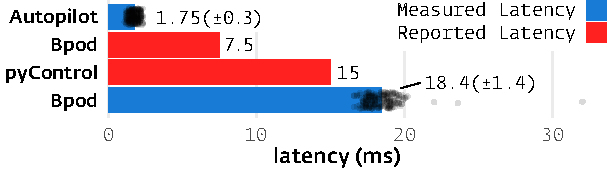
\includegraphics{figures/test_1_lags.pdf}
\end{figure}

\clearpage

Autopilot's  \texttt{1.75ms} $\pm$ \texttt{0.3} latency---less than 3x the theoretical minimum---improves upon the measured latency of Bpod and reported latency of pyControl by an order of magnitude (Figure \ref{fig:lags}, \texttt{18.4ms} $\pm$ \texttt{1.4}, \texttt{15ms} respectively). This suggests that Autopilot eliminates most perceptible end-to-end latency, which is necessary for tasks that require realtime feedback.

While we did not deeply investigate the reason why Bpod exceeded its theoretical minimum latency by more than 100x, potential sources of latency include a \href{https://github.com/sanworks/Bpod_Gen2/blob/825eaf6ea2cb11da956ee21c42876c4363e9c14e/Functions/Internal\%20Functions/ArCOM/ArCOMObject_Bpod.m#L304}{costly serial reading method}, or \href{https://github.com/sanworks/Bpod/blob/4b756d8251f0a06ee9a442e9cac465872c1b4174/Functions/RunStateMatrix.m#L189}{the MATLAB graphics engine being continuously called in the main loop of the program}, which are intrinsic to its single-threaded design.

Since Autopilot's event handling infrastructure is shared across tasks and hardware classes, latency for all events should be roughly similar to that of audio playback. One future direction is to improve upon Autopilot's already-low latency by compiling its sound server and event handling methods using Cython.

\section{Bandwidth}

\begin{margintable}[-6.6cm]
\caption{Terminal Specs}
\label{tab:terminal}
\noindent\begin{tabularx}{\linewidth}{rR}
\toprule
    CPU & AMD FX-4300 \\
    CPU Speed & 3.8GHz \\
    Memory & 8GB \\
    Ethernet & 1Gbit/s \\
    Switch & NETGEAR GSS116E \\
\bottomrule
\end{tabularx}
\end{margintable}

\begin{marginfigure}[-0.4cm]
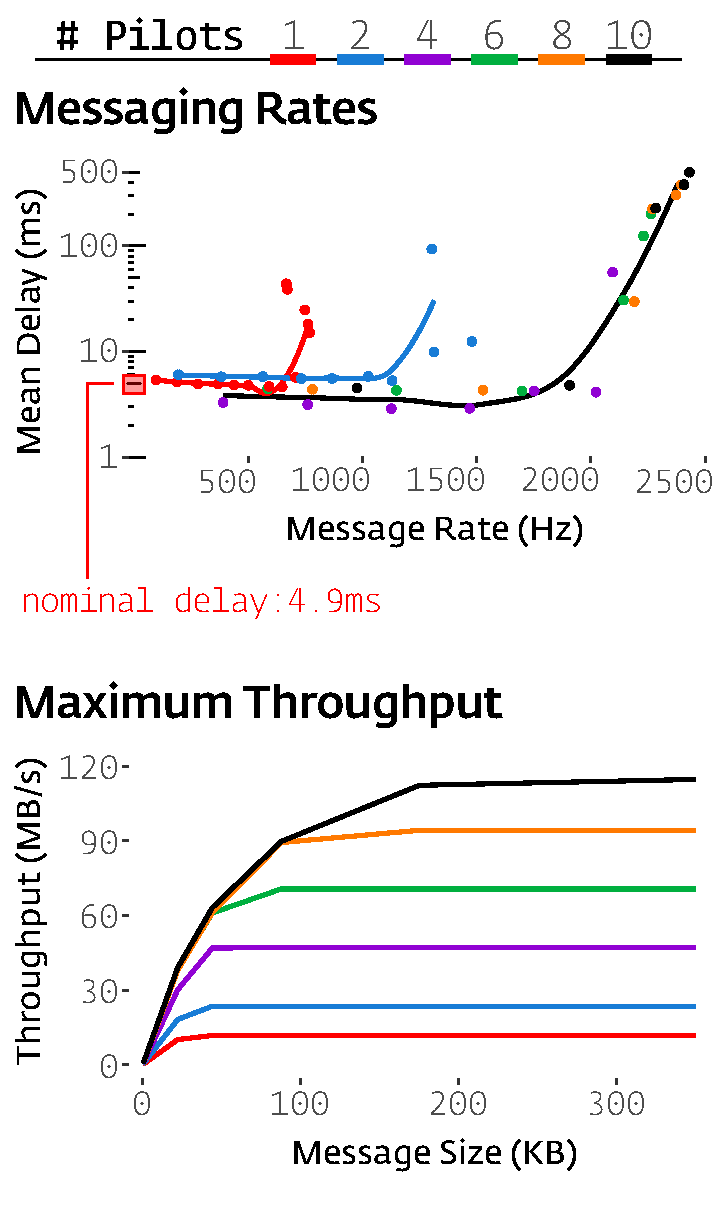
\includegraphics[]{figures/test_net_combined.pdf}

\caption{Network latency (top) and throughput (bottom) tests. Each point in the latency test represents the mean rate and delay of 5,000 255 Byte messages. Throughput (bottom) was calculated as the product of message rate and message size, and is displayed for a test that requested different numbers of pilots (colors) to send messages of different size to the terminal.}
\label{fig:speed}
\end{marginfigure}

To support data-intensive tasks like those that require online processing of video or electrophysiological data, the networking modules at the core of Autopilot need high bandwidth and low latency. 

We tested network capacity using Autopilot's \href{http://docs.auto-pi-lot.com/autopilot.core.gui.html#autopilot.core.gui.Bandwidth_Test}{\texttt{Bandwidth\_Test}} widget. This test requests that a set of selected pilots send messages at a range of selected frequencies and payload sizes back to the terminal. The messages pass through four networking objects en route: the stations and network nodes running the test for both the terminal and pilots (See Figure \ref{fig:datastreams}). Delay is measured as the duration between the creation of the message at the sender and the processing of the message at the receiver. The Pis and terminal were synchronized on common NTP servers to align timestamps. 

First we tested the limits of our terminal's ability to receive messages from the 10 pilots that it controls. Our terminal is a modest desktop (complete with a vintage 2012 CPU, see Table \ref{tab:terminal}) with ethernet connections to 10 Raspberry Pi 3b's through a network switch. We first tested the rate at which the Pi 3b's and our terminal could send and process typical (\texttt{255 Byte}) messages without a data payload (Figure \ref{fig:speed}, top). A single Pi was capable of sending at a maximum rate of \texttt{707 Hz} without exceeding its nominal mean delay of \texttt{4.9} ($\pm$ \texttt{0.47}) ms. Adding additional Pis did not cause increased delay until the total sending rate surpassed roughly \texttt{2000 Hz}. These are the rate limits of sending and receiving messages, respectively.

As we increased the size of each individual message by including payloads of generated data (Figure \ref{fig:speed}, bottom), the rate of messaging decreased, but the total throughput (\texttt{message rate (Hz) * size (Bytes)}) saturated linearly as a multiple of the number of sending Pis. The Raspberry Pi 3b has a shared USB/Ethernet Bus, and thus appears to have a relatively limited \texttt{11.8MB/s} throughput.

\begin{marginfigure}[0.1cm]
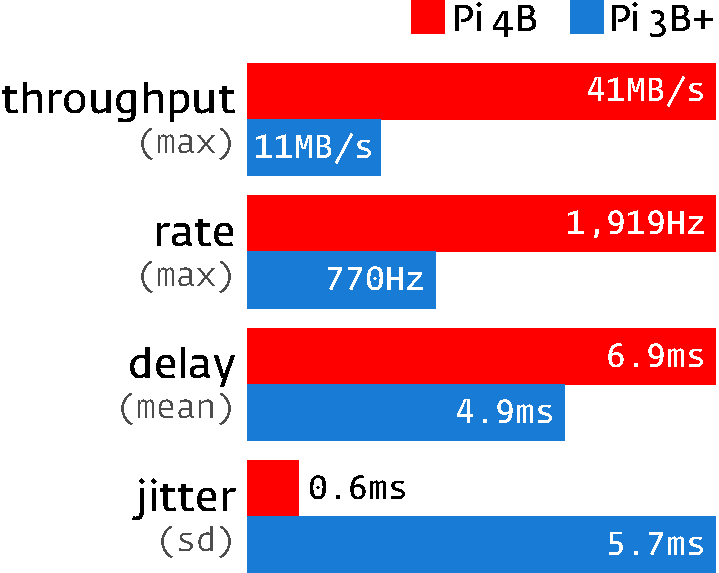
\includegraphics[]{figures/test_4_comparison.pdf}
\caption{The Raspberry Pi 4's gigabit ethernet bus markedly improves network performance.}
\label{fig:netcomparison}
\end{marginfigure}

Fortunately, the Raspberry Pi 4 has an independent \href{https://www.raspberrypi.org/magpi/raspberry-pi-4-specs-benchmarks/}{gigabit ethernet bus}. On a Raspberry Pi 4, Autopilot has a \texttt{41MB/s} maximum throughput and a \texttt{1,919Hz} maximum messaging rate (Figure \ref{fig:netcomparison}). We observed a slightly higher messaging delay with the Raspberry Pi 4 (\texttt{6.9ms} vs. \texttt{4.9ms} Raspberry Pi 3B+). We note that the NTP synchronization method we used to measure delays has a margin of error on the order of milliseconds. 

Autopilot's networking modules are capable of supporting the infrastructure of next-generation behavioral neuroscience experiments. Our humble terminal was capable of receiving the full \texttt{114.6MB/s} of 10 Pis without sign of saturation, and a Raspberry Pi 4 is capable of sending data at \texttt{41MB/s}. This bandwidth makes Autopilot capable of streaming raw Calcium imaging\sidenote{2-Photon:  5.9MB/s\\ \noindent (12 bits * 512x512 resolution * 15Hz)} and electrophysiological data from modern high-density probes\sidenote{Neuropixels: 14.4MB/s\citep{junFullyIntegratedSilicon2017}\\\noindent(10 bits * 30kHz * 384 channels)}. The delay between sending and processing messages over 4 hops in a network (\texttt{4.9ms}) is less than the latency with which comparable systems (Figure \ref{fig:lags}) process triggers when connected directly via serial.

Finally, while Autopilot typically operates in a "TCP-like" protocol---resending messages until they have been confirmed as received---these tests were run with an optional "UDP-like" protocol which does not check for confirmation. Across the approximately 2.5 million messages sent during these tests only \texttt{537} were dropped (and only during tests which saturated rate or bandwidth capacity), giving Autopilot a delivery rate of \texttt{99.98\%} in "UDP" mode. By design, delivery rate is guaranteed to be 100\% in "TCP" mode.
